% Copyright 2004 by Till Tantau <tantau@users.sourceforge.net>.
%
% In principle, this file can be redistributed and/or modified under
% the terms of the GNU Public License, version 2.
%
% However, this file is supposed to be a template to be modified
% for your own needs. For this reason, if you use this file as a
% template and not specifically distribute it as part of a another
% package/program, I grant the extra permission to freely copy and
% modify this file as you see fit and even to delete this copyright
% notice. 

\documentclass{beamer}

\usepackage{floatrow}%

% There are many different themes available for Beamer. A comprehensive
% list with examples is given here:
% http://deic.uab.es/~iblanes/beamer_gallery/index_by_theme.html
% You can uncomment the themes below if you would like to use a different
% one:
%\usetheme{AnnArbor}
%\usetheme{Antibes}
%\usetheme{Bergen}
%\usetheme{Berkeley}
%\usetheme{Berlin}
%\usetheme{Boadilla}
%\usetheme{boxes}
%\usetheme{CambridgeUS}
%\usetheme{Copenhagen}
%\usetheme{Darmstadt}
%\usetheme{default}
%\usetheme{Frankfurt}
%\usetheme{Goettingen}
%\usetheme{Hannover}
%\usetheme{Ilmenau}
%\usetheme{JuanLesPins}
%\usetheme{Luebeck}
\usetheme{Madrid}
%\usetheme{Malmoe}
%\usetheme{Marburg}
%\usetheme{Montpellier}
%\usetheme{PaloAlto}
%\usetheme{Pittsburgh}
%\usetheme{Rochester}
%\usetheme{Singapore}
%\usetheme{Szeged}
%\usetheme{Warsaw}

\title{3D Reconstruction From Shadows}

\author{Emile Okada\inst{1}}
% - Give the names in the same order as the appear in the paper.
% - Use the \inst{?} command only if the authors have different
%   affiliation.

\institute[University of Cambridge] % (optional, but mostly needed)
{
  \inst{1}%
  DAMTP\\
  University of Cambridge
  }
% - Use the \inst command only if there are several affiliations.
% - Keep it simple, no one is interested in your street address.

\date{Group meeting}
% - Either use conference name or its abbreviation.
% - Not really informative to the audience, more for people (including
%   yourself) who are reading the slides online

\subject{Image Analysis}
% This is only inserted into the PDF information catalog. Can be left
% out. 

% If you have a file called "university-logo-filename.xxx", where xxx
% is a graphic format that can be processed by latex or pdflatex,
% resp., then you can add a logo as follows:

% \pgfdeclareimage[height=0.5cm]{university-logo}{university-logo-filename}
% \logo{\pgfuseimage{university-logo}}

% Delete this, if you do not want the table of contents to pop up at
% the beginning of each subsection:
\AtBeginSubsection[]
{
  \begin{frame}<beamer>{Outline}
    \tableofcontents[currentsection,currentsubsection]
  \end{frame}
}

% Let's get started
\begin{document}

\begin{frame}
  \titlepage
\end{frame}

\begin{frame}{Outline}
  \tableofcontents
  % You might wish to add the option [pausesections]
\end{frame}

\section{Motivation}

\begin{frame}{Motivation}
    \begin{figure}[H]
      \centering
        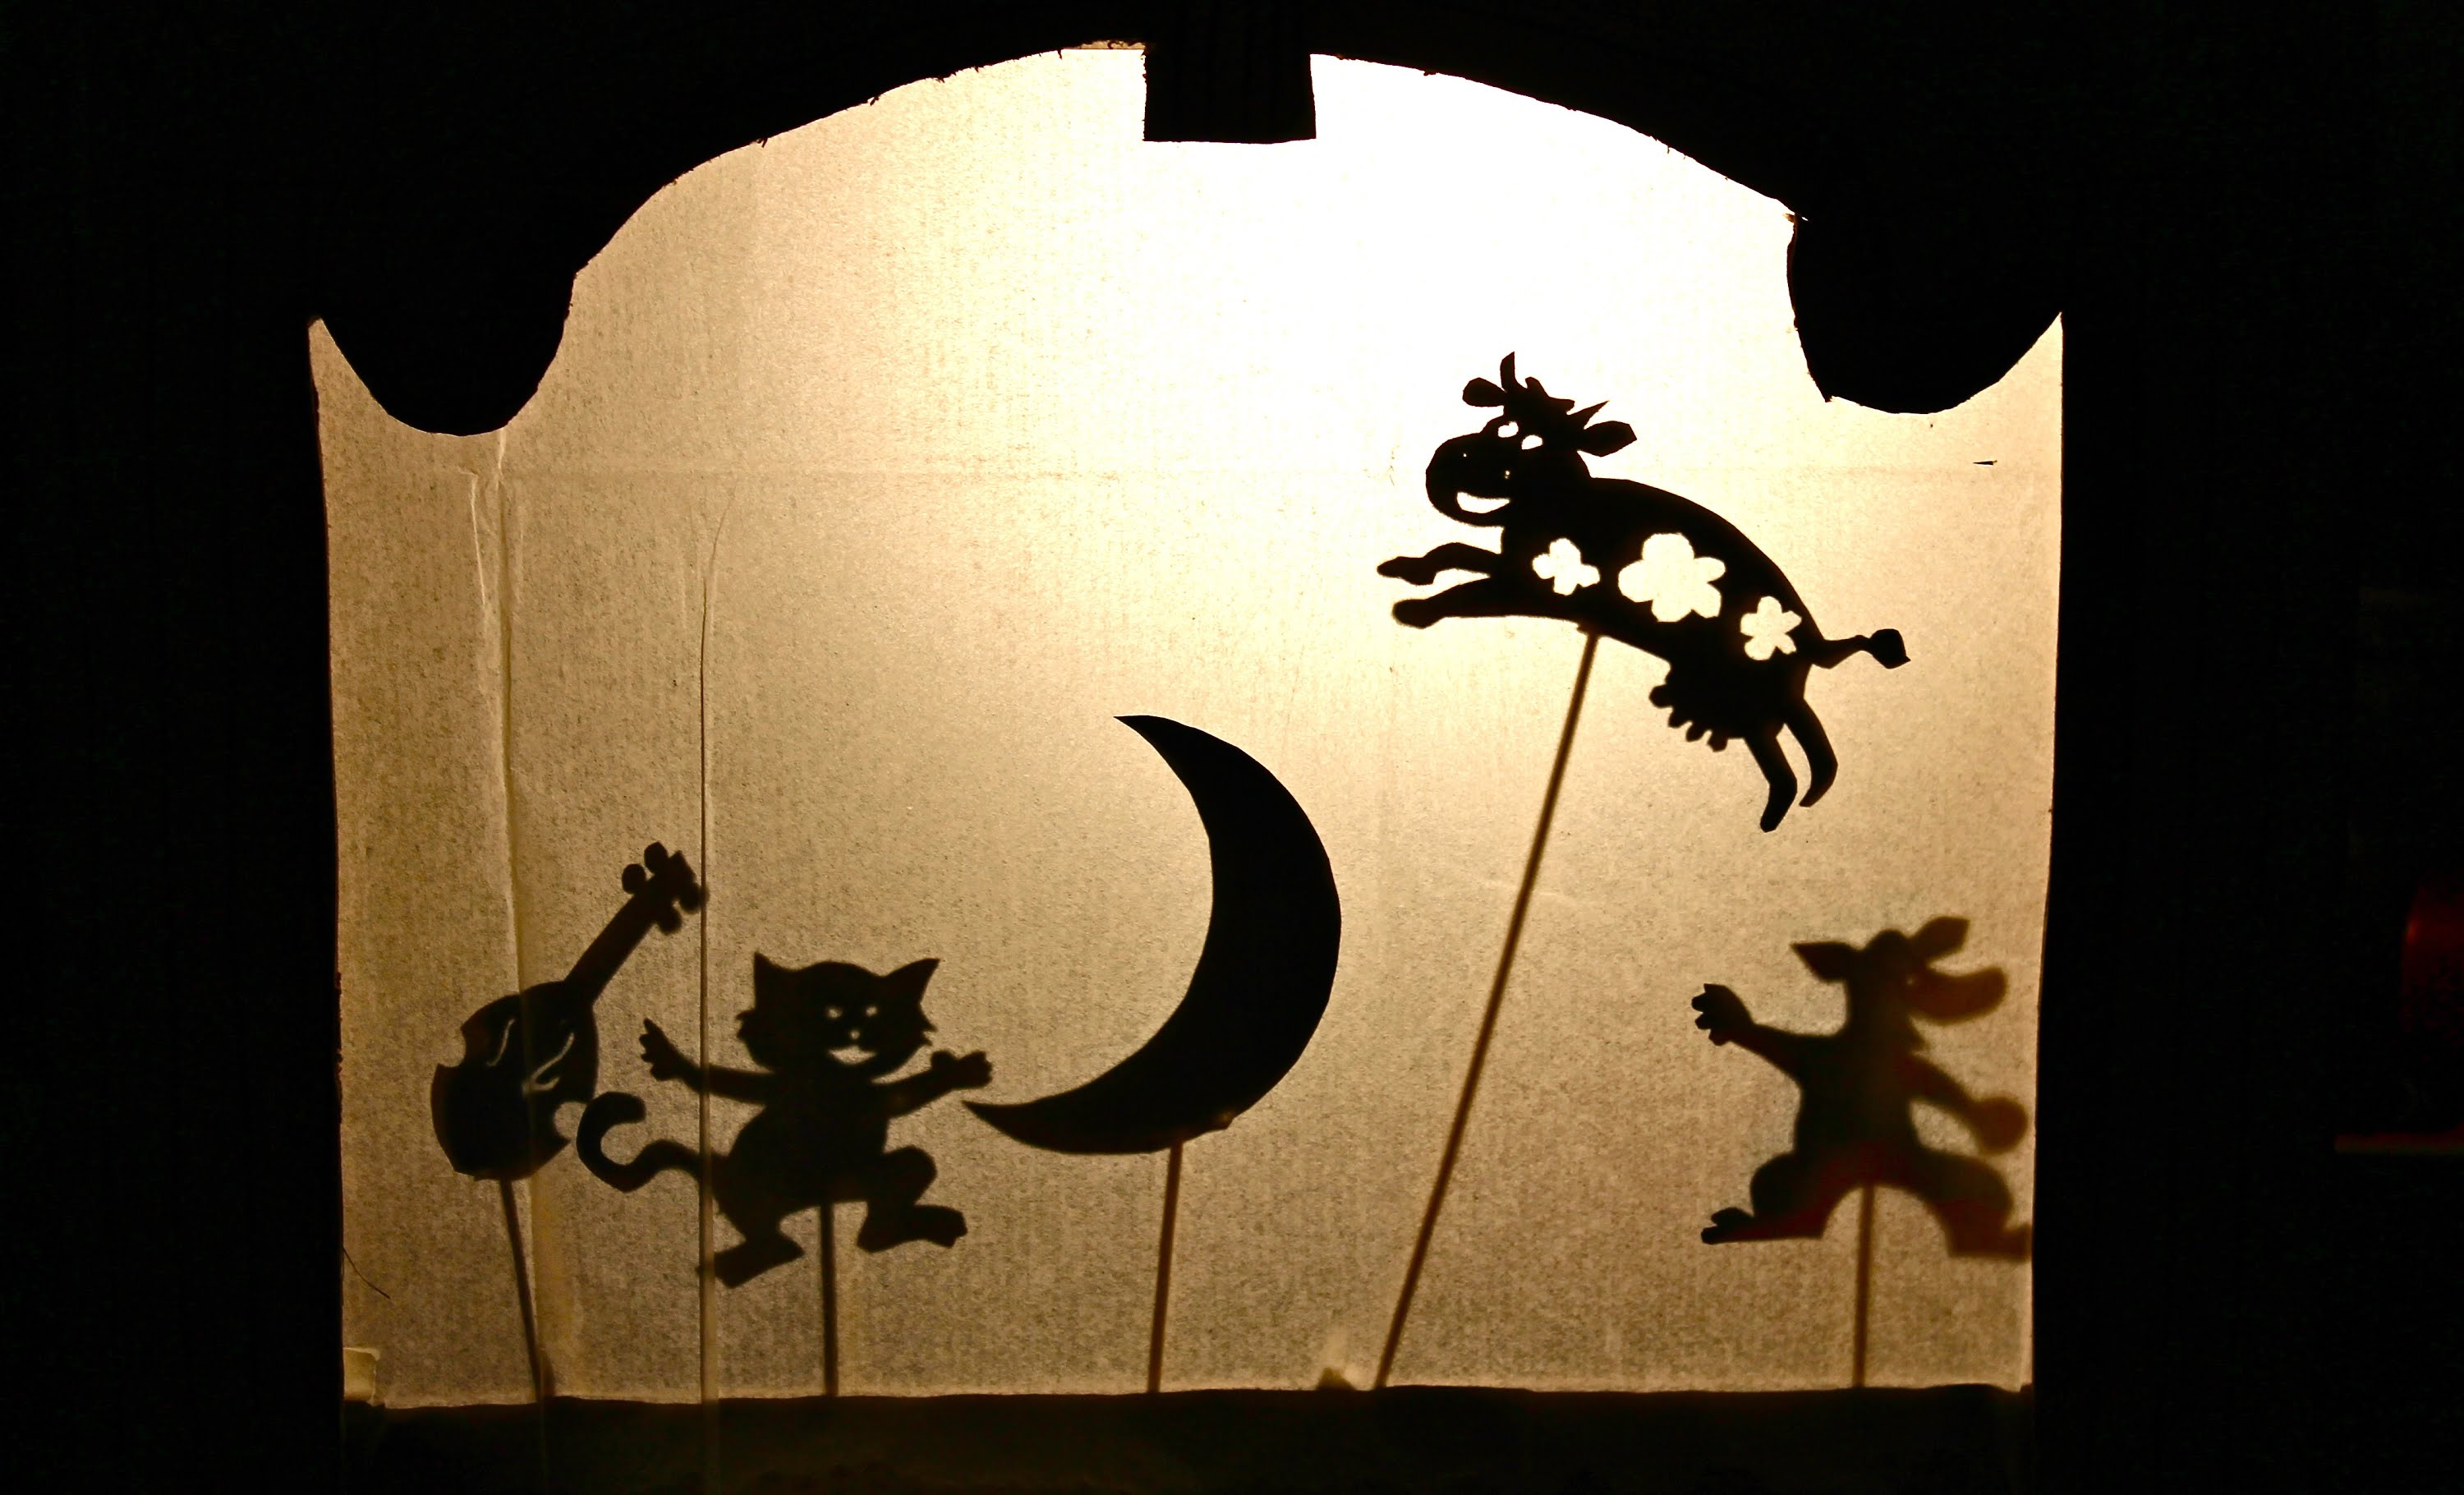
\includegraphics[width=0.8\textwidth]{puppets.jpg}
      \label{fig:f2}
    \end{figure}
\end{frame}

% Section and subsections will appear in the presentation overview
% and table of contents.
\section{2D Reconstructions}

\subsection{What kind of sets can we reconstruct?}

\begin{frame}{What kind of sets can we reconstruct?}
    \begin{figure}[H]
        \begin{floatrow}
            \ffigbox{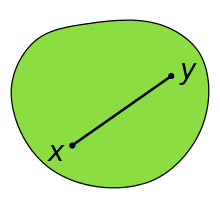
\includegraphics[scale = 0.5]{convex.png}}{\label{fig:err1}}
            \ffigbox{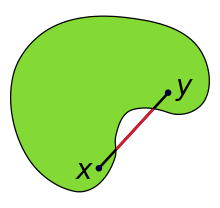
\includegraphics[scale = 0.5]{non_convex.png}}{\label{fig:err2}}
        \end{floatrow}
    \end{figure}
\end{frame}

\subsection{How to perform the reconstruction}

% You can reveal the parts of a slide one at a time
% with the \pause command:
\begin{frame}{Cautionary tale}
    \begin{figure}[H]
      \centering
        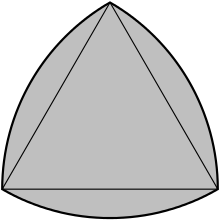
\includegraphics[width=0.5\textwidth]{const_width.png}
      \label{fig:f2}
    \end{figure}
\end{frame}

\begin{frame}{Example}
    \begin{figure}[H]
        \begin{floatrow}
            \ffigbox{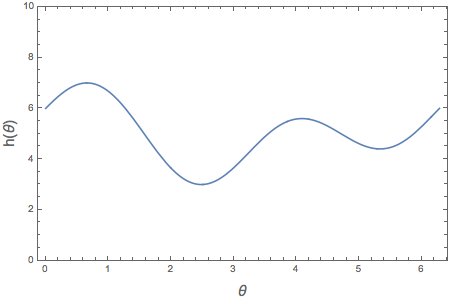
\includegraphics[scale = 0.3]{h.png}\caption{Shadow function}}{\label{fig:err3}}
            \ffigbox{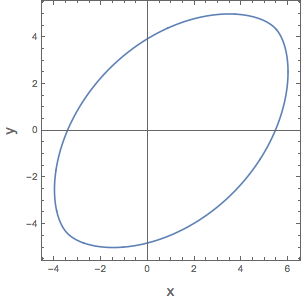
\includegraphics[scale = 0.3]{d.png}\caption{Reconstructed domain}}{\label{fig:err4}}
        \end{floatrow}
    \end{figure}
\end{frame}

\section{3D Reconstructions}

\subsection{'Slice-wise' convex volumes}

\begin{frame}{3D Reconstruction}
    \begin{figure}[H]
      \centering
        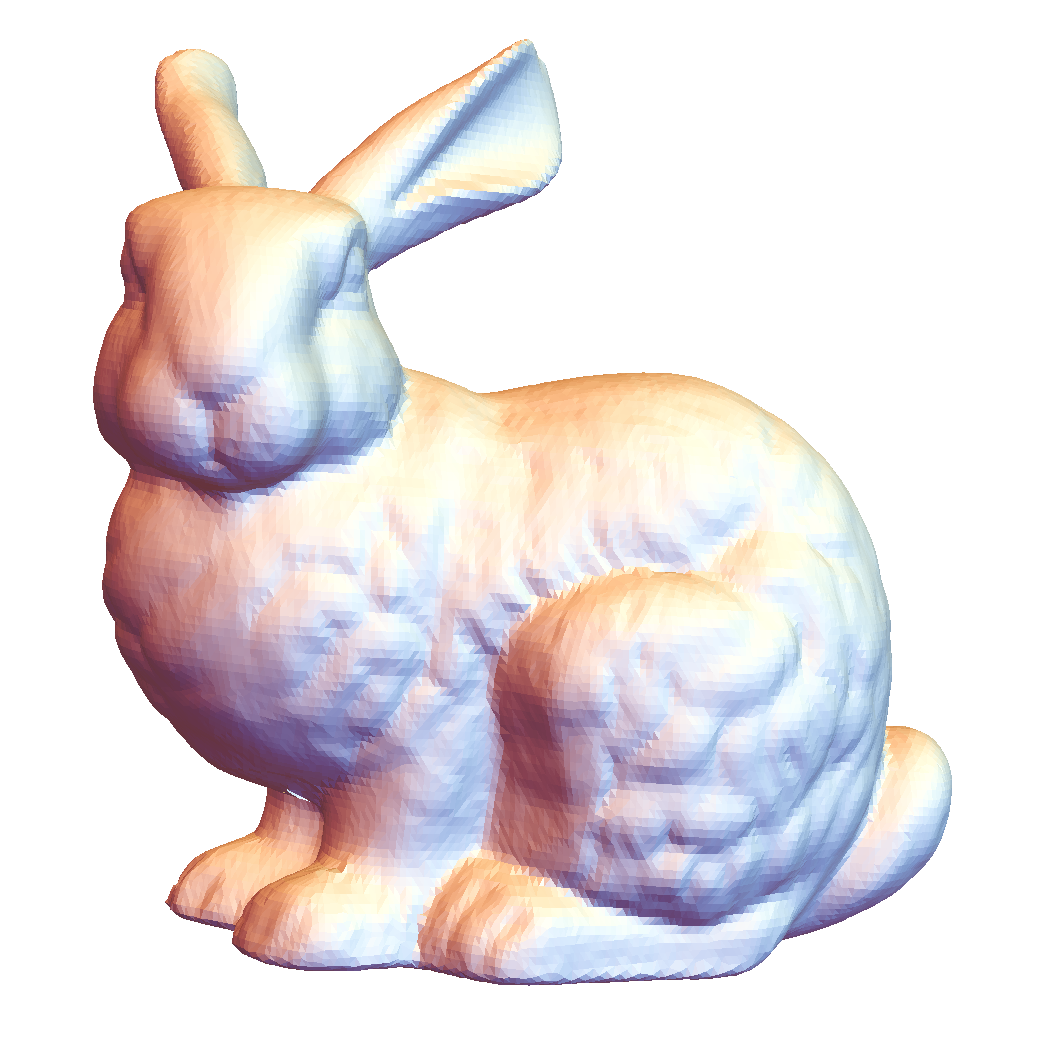
\includegraphics[width=0.5\textwidth]{3D_rabit.png}
      \label{fig:f2}
    \end{figure}
\end{frame}

\begin{frame}{3D Reconstruction}
    \begin{figure}[H]
        \begin{floatrow}
            \ffigbox{
\includegraphics[scale = 0.4]{rabit1.jpg}}{\label{fig:err5}}
            \ffigbox{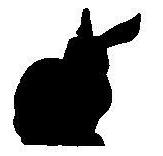
\includegraphics[scale = 0.4]{rabit4.jpg}}{\label{fig:err6}}
        \end{floatrow}
    \end{figure}
    \begin{figure}[H]
        \begin{floatrow}
            \ffigbox{
\includegraphics[scale = 0.4]{rabit7.jpg}}{\label{fig:err7}}
            \ffigbox{
\includegraphics[scale = 0.4]{rabit10.jpg}}{\label{fig:err8}}
        \end{floatrow}
    \end{figure}
\end{frame}

\begin{frame}{3D Reconstruction}
    \begin{figure}[H]
      \centering
        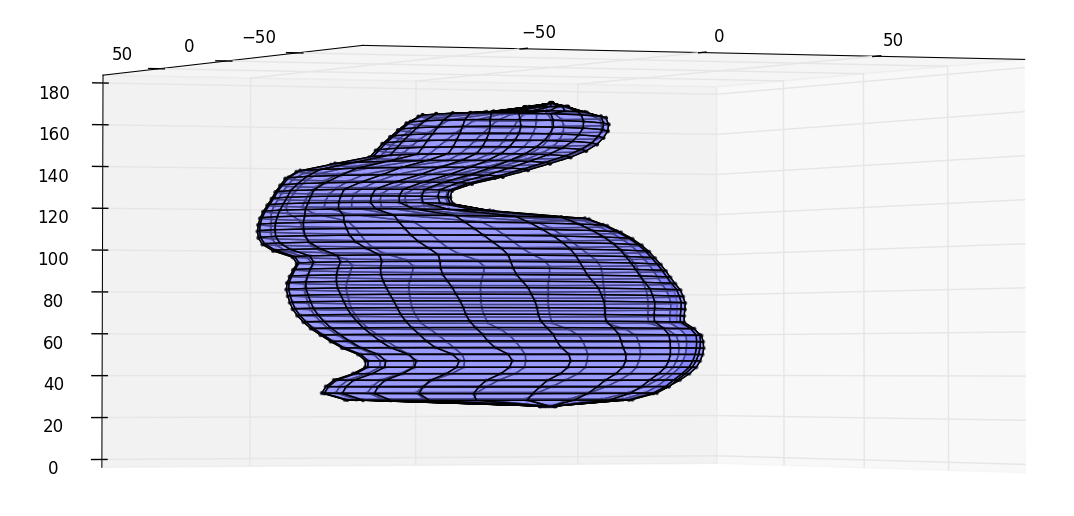
\includegraphics[width=0.8\textwidth]{polygonal_mesh.png}
      \label{fig:f2}
    \end{figure}
\end{frame}

\begin{frame}{But the ears!}
    \begin{figure}[H]
        \begin{floatrow}
            \ffigbox{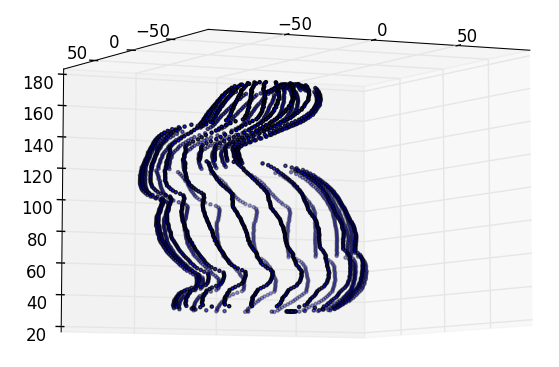
\includegraphics[scale = 0.4]{rabit.png}}{\label{fig:err7}}
            \ffigbox{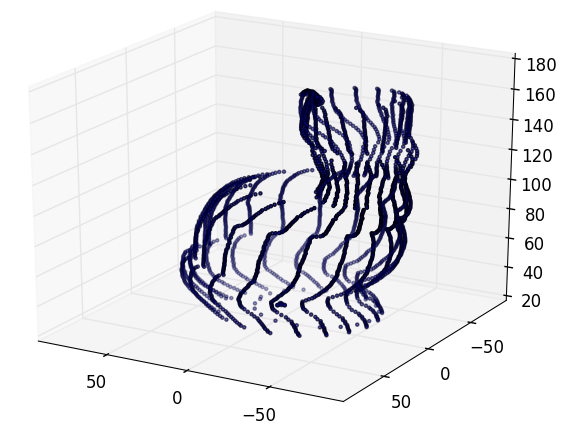
\includegraphics[scale = 0.4]{ear_and_back_cutoff.png}}{\label{fig:err8}}
        \end{floatrow}
    \end{figure}
\end{frame}

\begin{frame}{3D Reconstruction}
    \begin{figure}[H]
        \begin{floatrow}
            \ffigbox{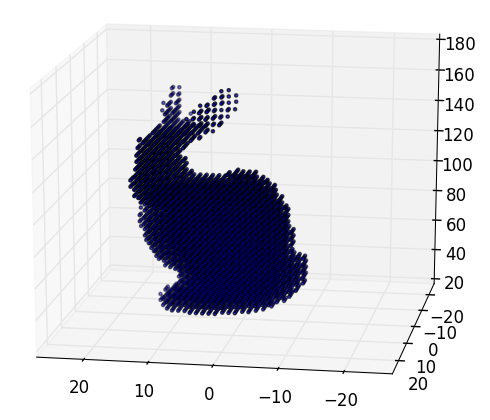
\includegraphics[scale = 0.4]{rabit_ears_3.png}}{\label{fig:err9}}
            \ffigbox{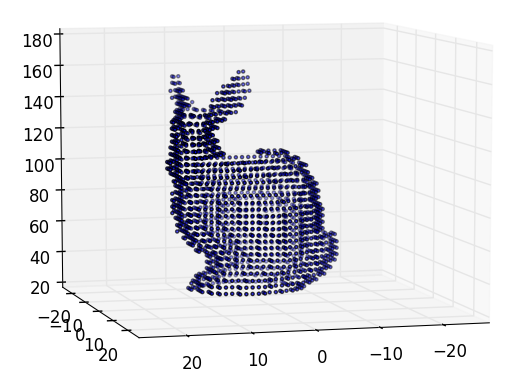
\includegraphics[scale = 0.4]{rabit_ears_4.png}}{\label{fig:err10}}
        \end{floatrow}
    \end{figure}
\end{frame}

\section{TV Denoising}

\begin{frame}{TV Denoising}
    \begin{equation}
        \min_{u}\int_{\Omega}|Du|+\frac12\lambda \|u-f\|_2^2 \nonumber
    \end{equation}
\end{frame}

\end{document}


